% =========================================================================
\documentclass[notes, aspectratio=1610]{beamer}
%\documentclass[aspectratio=1610]{beamer}

% ========================= Theme =========================================
\usetheme{Berkeley}
\usecolortheme{seahorse}

% ========================= Essential packages ============================
%\usepackage{hyperref}
%\hypersetup{
%    colorlinks = true,
%    linkcolor = blue,
%    citecolor = blue,
%    filecolor = blue,
%    urlcolor = blue
%}

% ========================= Frame notes systm ============================
%\usepackage{pgfpages}
%\setbeameroption{show notes on second screen}

% ========================= Plotting ======================================
\usepackage{calc}
\usepackage{tikz}
\usetikzlibrary{arrows,
                arrows.meta,
                calc,
		chains,
                quotes,
                positioning,
		shapes,
                shapes.geometric}
\usepackage{graphicx}
\usepackage{graphics}
\usepackage{pgfplots}
\pgfplotsset{width=7cm,compat=1.17}

%% ============================== Tabular =================================
\usepackage{booktabs}
\usepackage{tabularx,ragged2e}
\usepackage{array}
\usepackage{multirow}
\usepackage{siunitx}
  \sisetup{detect-all}
\usepackage{adjustbox}
\usepackage{rotating}
\usepackage{threeparttable}
\usepackage[justification=centering]{caption}
\usepackage{color, colortbl}

%% ============================== Text boxes ==============================
\usepackage[most]{tcolorbox}		

% ========================= Infor on authors ==============================
%\title[Visualization Design]%
%{Visualization Design}
\title{Interactive Visualization}
\author{S.~Santoni\inst{1}\inst{2}}
\institute{
	\inst{1}%
	Bayes Business School
	\and
	\inst{2}%
	Soundcloud
	}
\date{MSc in Business Analytics, 2022/23}

% ============================ Colors =====================================
\definecolor{base_c}{rgb}{0.6,0,0}
\definecolor{comp_c}{rgb}{0.09803921568627451, 0.6901960784313725, 0.7529411764705882}
\definecolor{tri_1}{rgb}{0.09803921568627451, 0.7686274509803922, 0.19215686274509805}
\definecolor{tri_2}{rgb}{0.19215686274509805, 0.09803921568627451, 0.7686274509803922}

% ========================= TOC  ==========================================
\AtBeginSection[]
{
	\begin{frame}
		       \frametitle{Outline}
		       \tableofcontents[currentsection,currentsubsection]
	\end{frame}
}

% ========================= References ===================================
\usepackage[style=numeric,backend=biber]{biblatex}
\addbibresource{bibliography.bib}

% ========================= Document  ====================================
\begin{document}

\begin{frame}
	\titlepage
\end{frame}

\begin{frame}{Outline}
	\tableofcontents
\end{frame}

% ========================= Week 4 wrap up =================================
\section{Session \#4 Wrap Up}

\begin{frame}{Designing the `Lower-Level' Features of a Chart}
	{Source \cite[][page 61]{cairo2012}}
	\centering 
	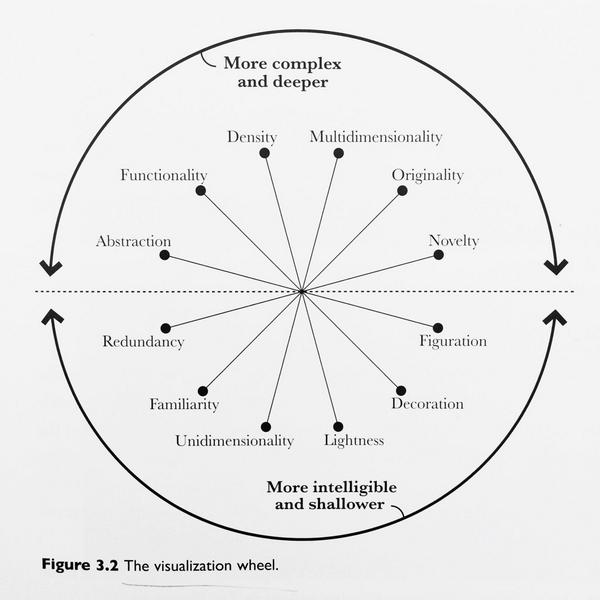
\includegraphics[width=0.55\textwidth]{images/viz_wheel.jpeg}
\end{frame}

\begin{frame}{Designing the `Lower-Level' Features of a Chart}
	{Source \cite[][page 63]{cairo2012}}
	\centering 
	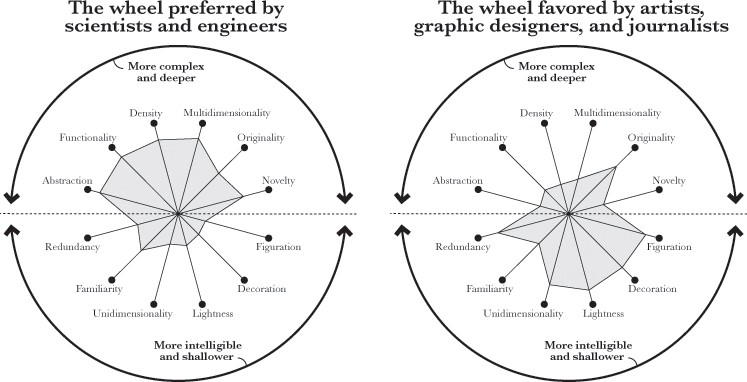
\includegraphics[width=0.9\textwidth]{images/viz_whell_comparison.jpeg}
\end{frame}

\begin{frame}{Chartjunk?}{}
	\centering 
	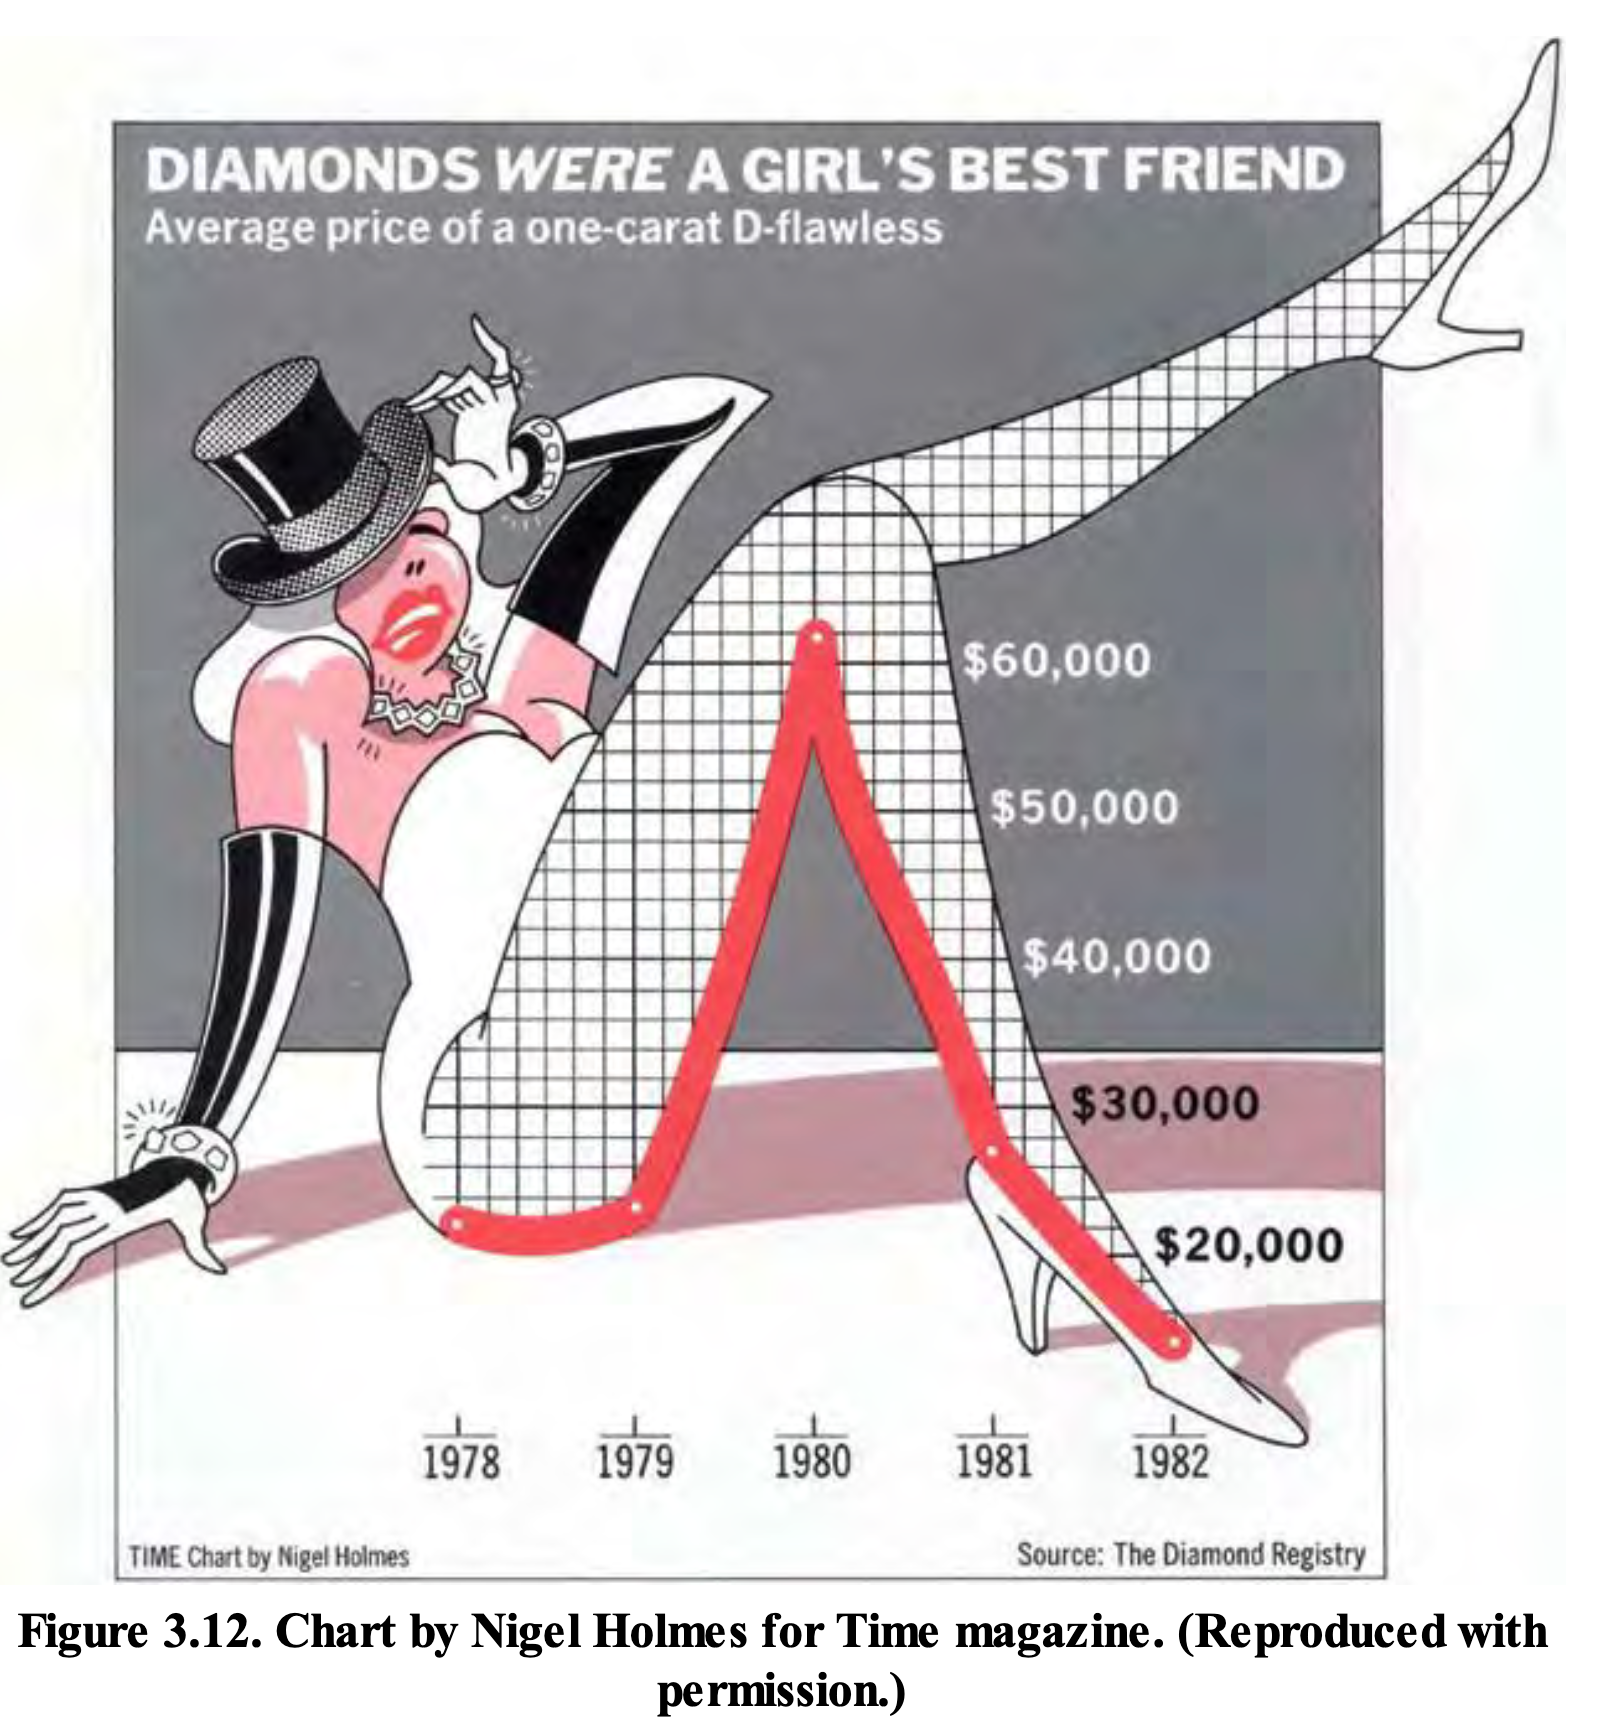
\includegraphics[width=0.55\textwidth]{images/chartjunk.png}
\end{frame}

\begin{frame}{Chartjunk or Memorable?}{}
	\centering 
	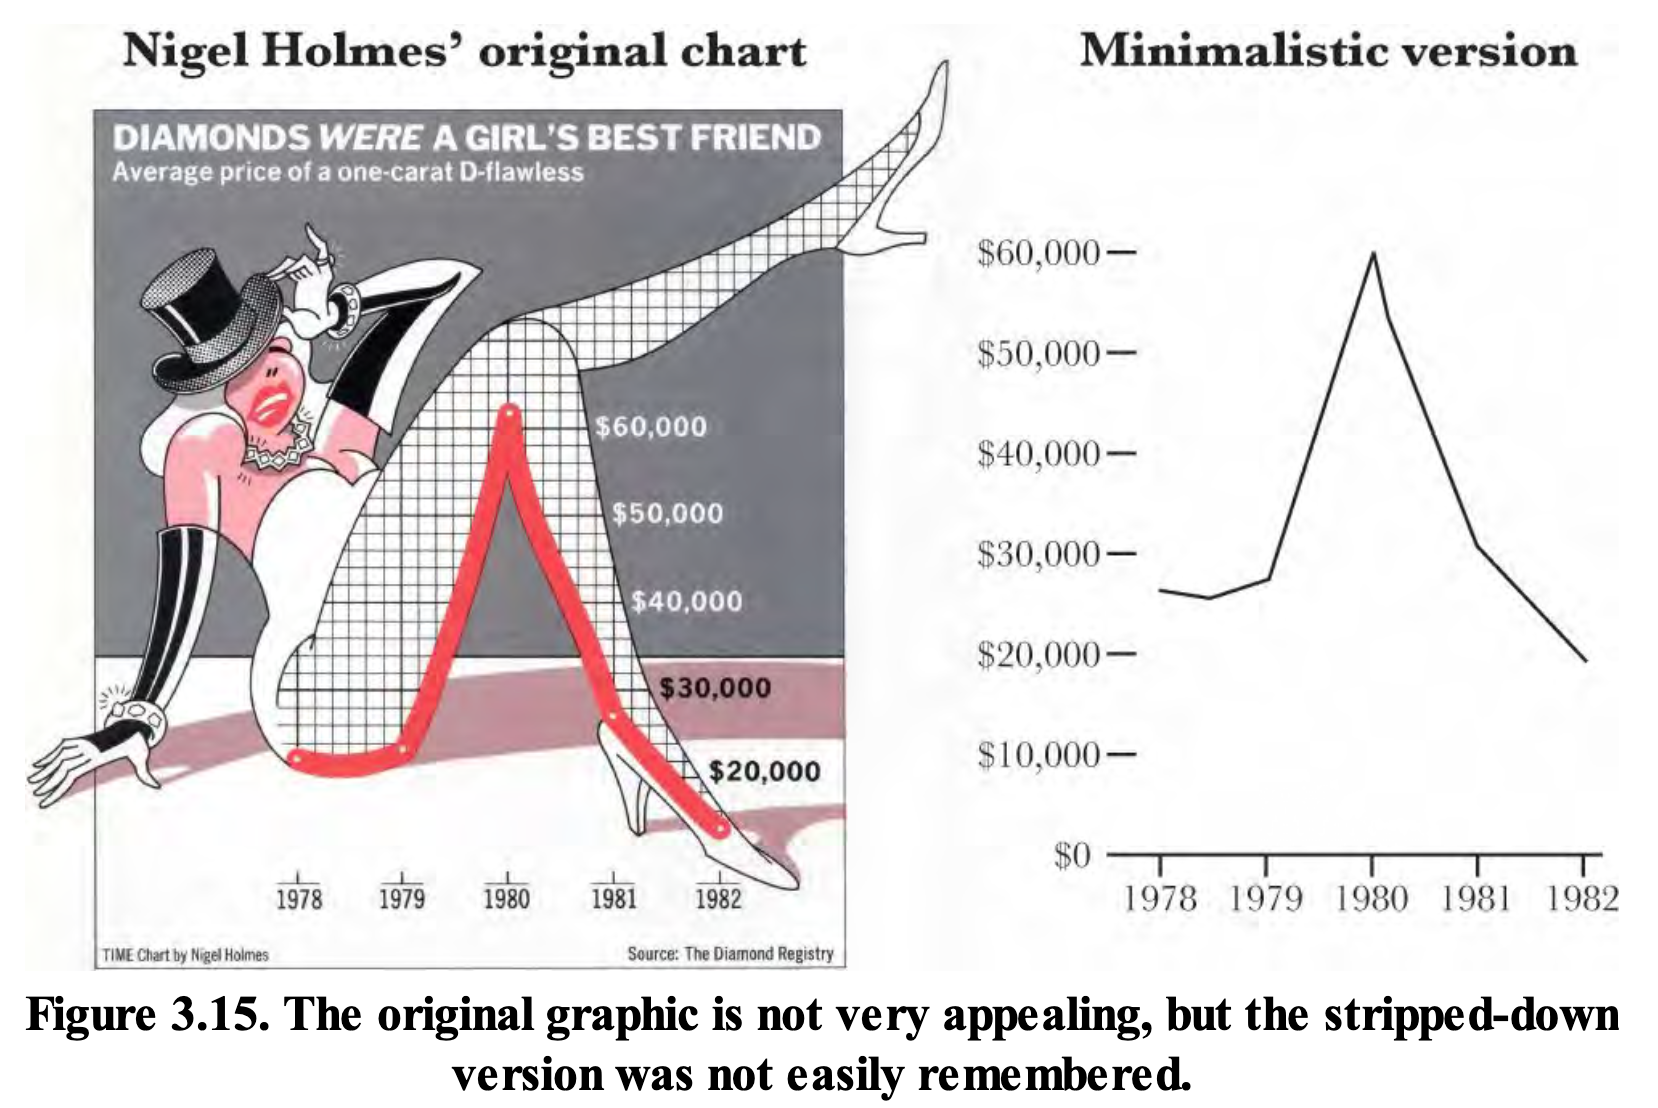
\includegraphics[width=0.8\textwidth]{images/chartjunk_vs_tufter.png}
\end{frame}

\begin{frame}{}{}
	\centering
	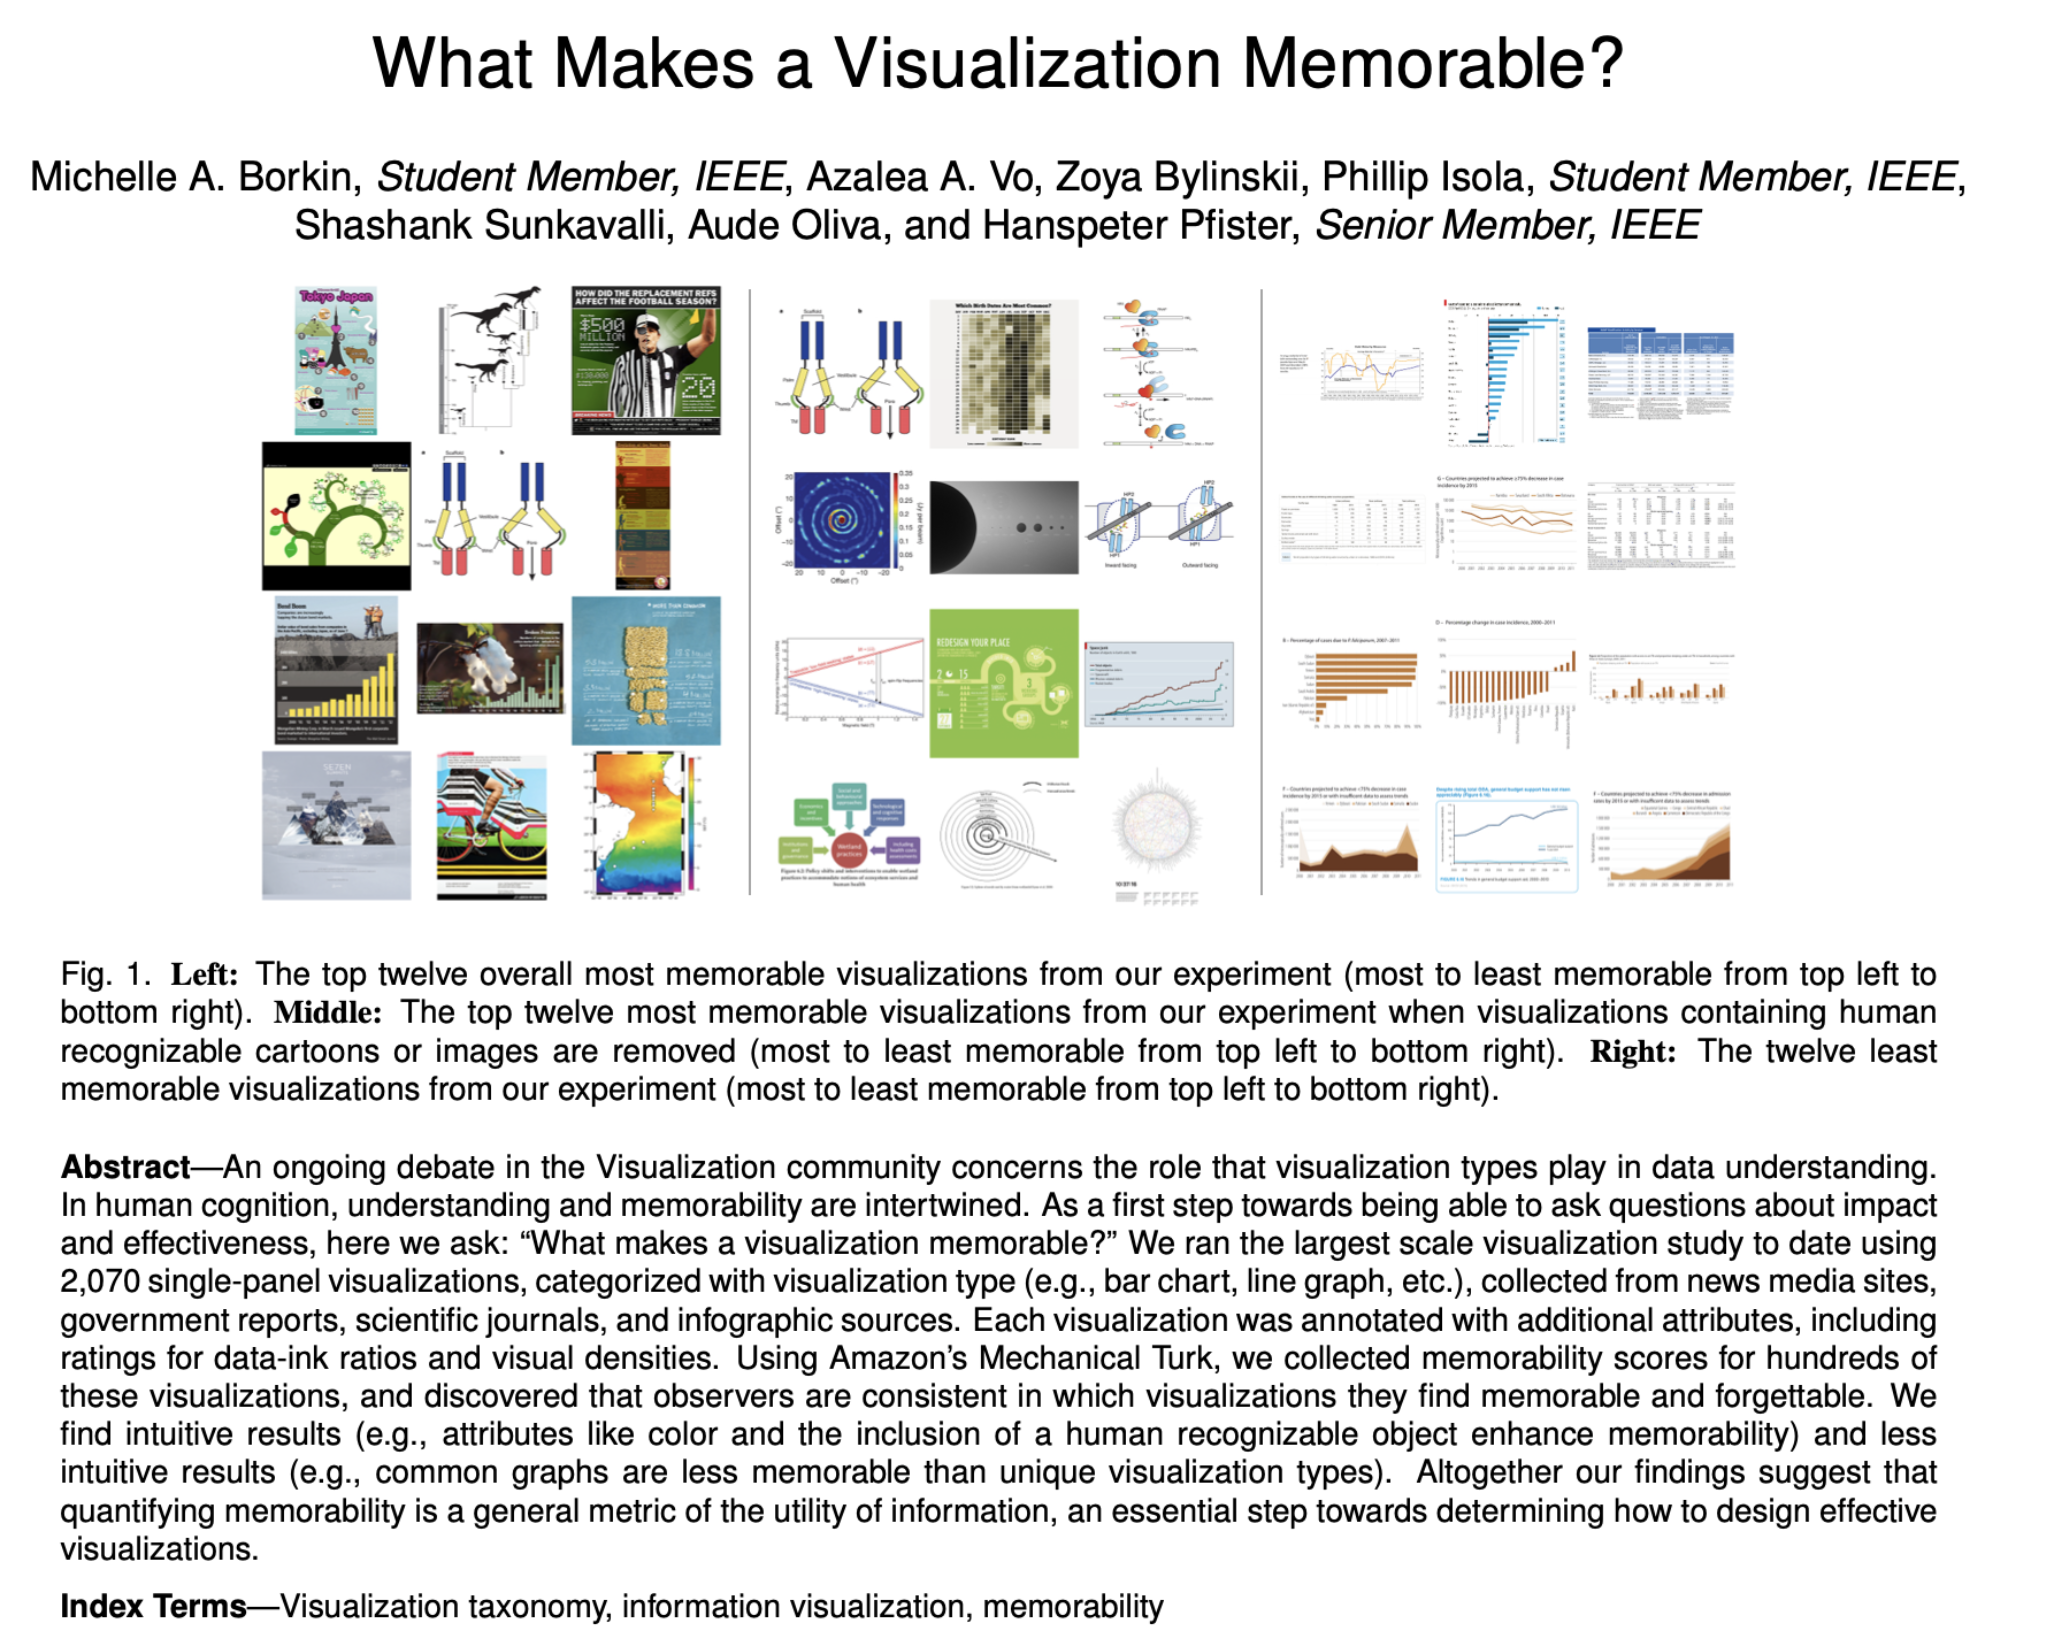
\includegraphics[width=0.7\textwidth]{images/memorable_data_viz.png}
\end{frame}

\begin{frame}{Empirical Evidence on Visualization Memorability}
	{The role of pictograms}
	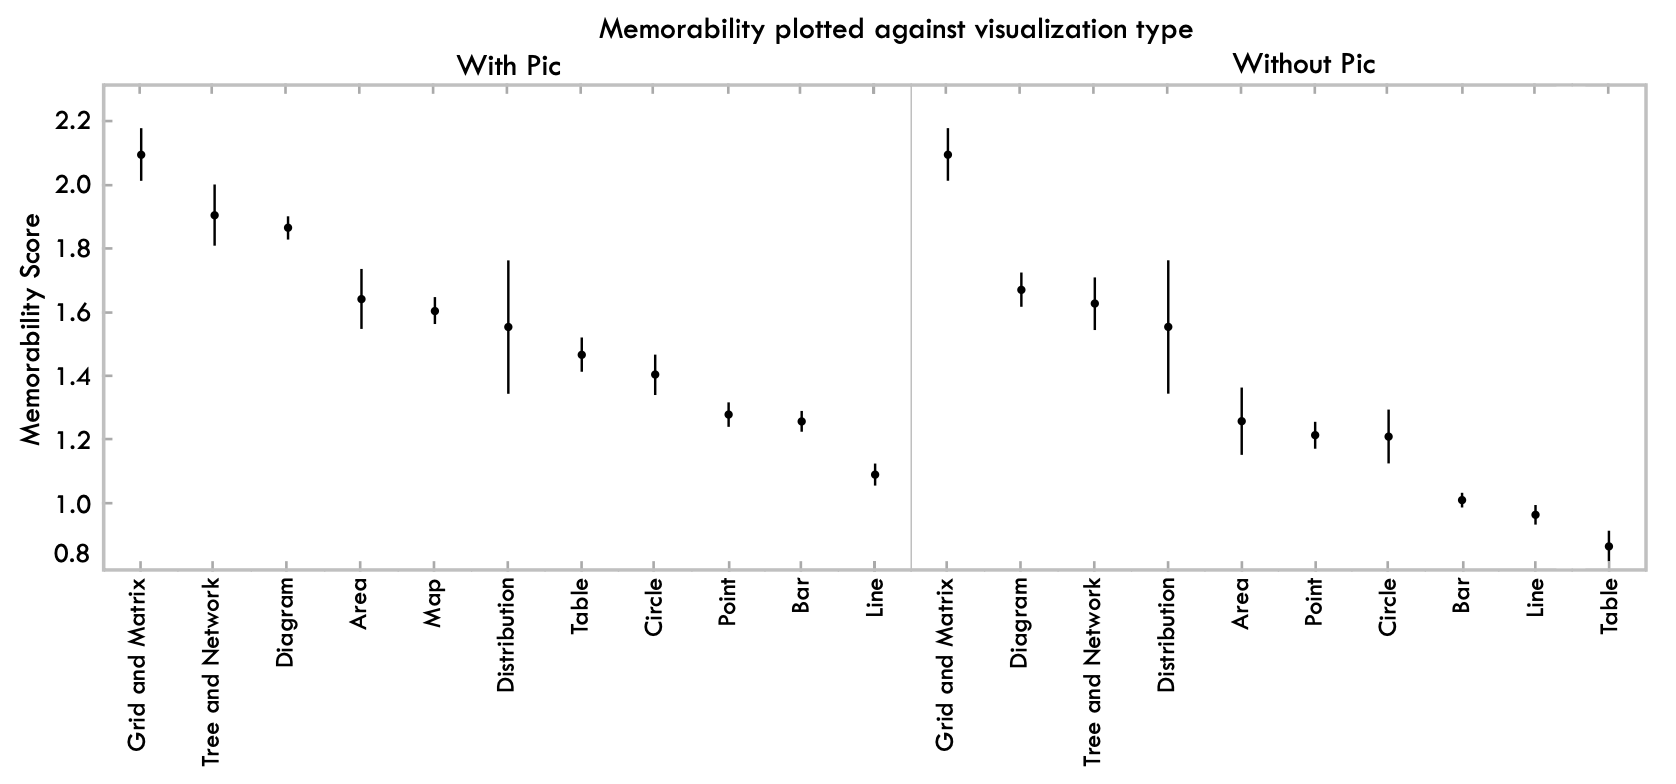
\includegraphics[width=1\textwidth]{images/1_4}
\end{frame}

\begin{frame}{Empirical Evidence on Visualization Memorability}
	{The role of pictograms and color rating}
	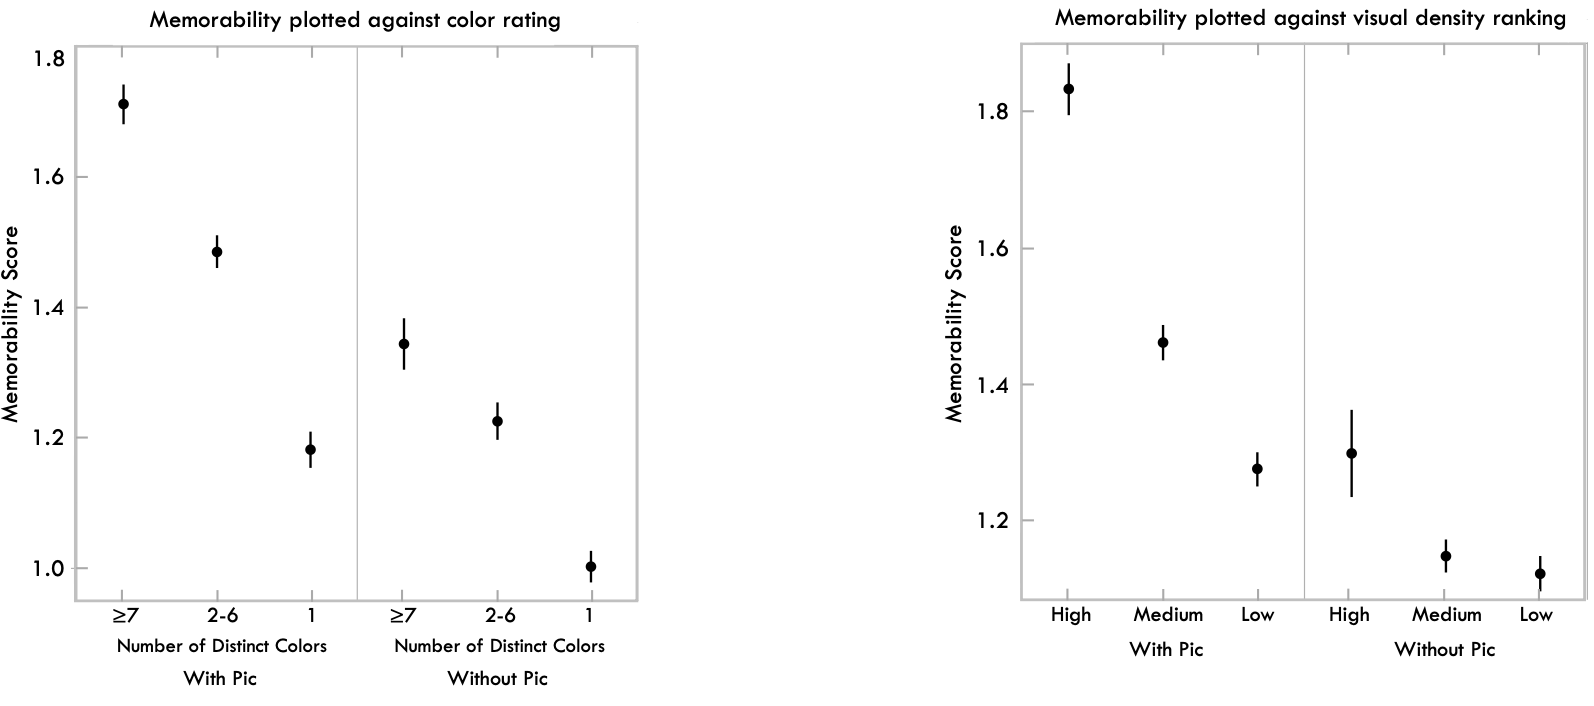
\includegraphics[width=1\textwidth]{images/2_4}
\end{frame}

\begin{frame}{Empirical Evidence on Visualization Memorability}
	{The role of data-ink ratio and pictograms}
	\centering
	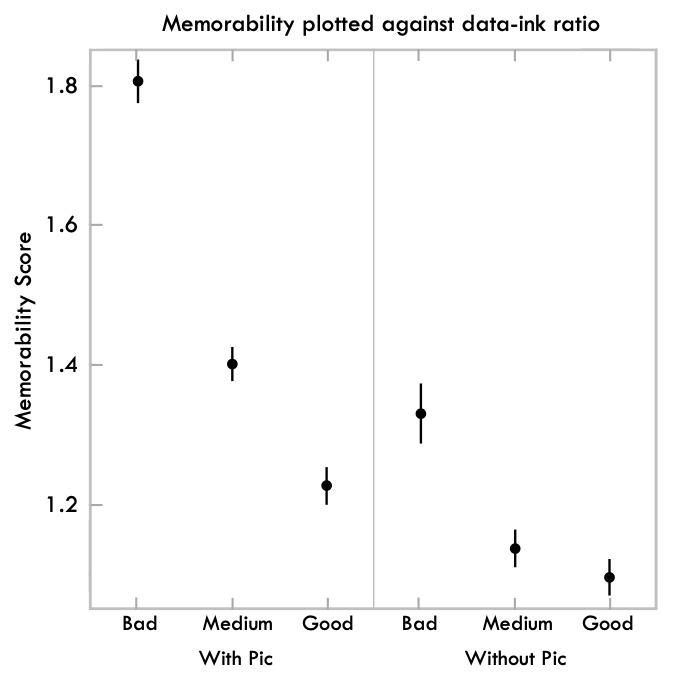
\includegraphics[width=0.6\textwidth]{images/3_4}
\end{frame}

\begin{frame}{Empirical Evidence on Visualization Memorability}
	{The role of pictograms and source}
	\centering
	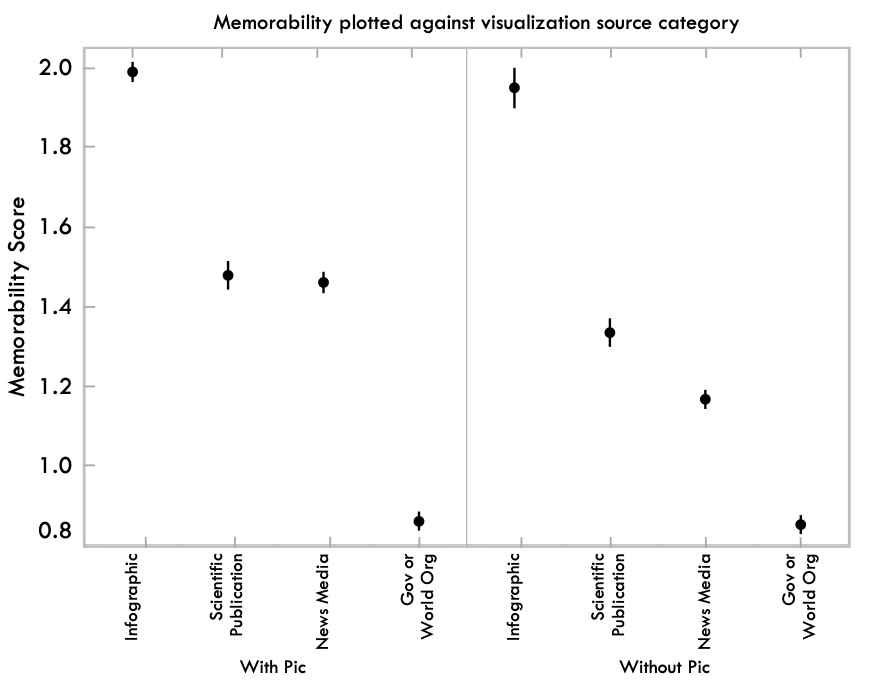
\includegraphics[width=0.7\textwidth]{images/4_4}
\end{frame}

% ========================== Interactive dynamics and data viz =============
\section{Interactive Dynamics and Data Visualization}

\begin{frame}{From Static to Dynamic Visualization}{}
	\begin{center}
		\textbf{How to escape flatland?}
	\end{center}
	
	A single image typically provides answers to, at best, a handful of 
	questions

	\vspace{2em}

	\pause

\begin{columns}
	\begin{column}{0.5\textwidth}
		\begin{center}
			\textbf{Dynamic viz is my solution!}
		\end{center}

		Meaningful analysis consists of repeated explorations as users
		develop insights about significant relationships,
		domain-specific contextual influences, and causal patterns
	\end{column}

	\pause

	\begin{column}{0.5\textwidth}

		\begin{center}
			\textbf{Hold on...maybe not...}
		\end{center}
		Confusing widgets, complex dialog boxes, hidden operations,
		incomprehensible displays, or slow response times can limit the
		range and depth of topics considered and may curtail thorough
		deliberation and introduce errors
	\end{column}
\end{columns}

\end{frame}

\begin{frame}{A Taxanomy of Interactive Dynamics for Visual Analysis}{}
	\footnotesize
	\centering
	\begin{table}
		\begin{tabular}{l|l}
			\hline
			\rowcolor{gray!25}
			Data \& View Specification
			%$\bullet$ Visualize data by choosing visual encodings \\
			%\rowcolor{gray!25}
			& $\bullet$ Filter out data to focus on relevant items\\
			\rowcolor{gray!25}
			& $\bullet$ Sort items to expose patterns\\
			\rowcolor{gray!25} 
			& $\bullet$ Derive values or models from source data \\
			\hline
			View Manipulation
			& $\bullet$ Select items to highlight, filter, or manipulate them \\
			& $\bullet$ Navigate to examine high-level patterns and low-level detail\\
			& $\bullet$ Coordinate views for linked, multi-dimensional exploration\\ 
			& $\bullet$ Organize multiple windows and workspaces\\
			\hline
			\rowcolor{gray!25}
			Process \& Provenance
			& $\bullet$ Record analysis histories for revisitation, review and sharing\\
			\rowcolor{gray!25}
			& $\bullet$ Annotate patterns to document findings\\
			\rowcolor{gray!25}
			& $\bullet$ Share views and annotations to enable collaboration\\
			\rowcolor{gray!25}
			& $\bullet$ Guide users through analysis tasks or stories\\
			\hline
		\end{tabular}
	\end{table}
\end{frame}

\begin{frame}{Let Us Get Things Done!}{}
	\centering
	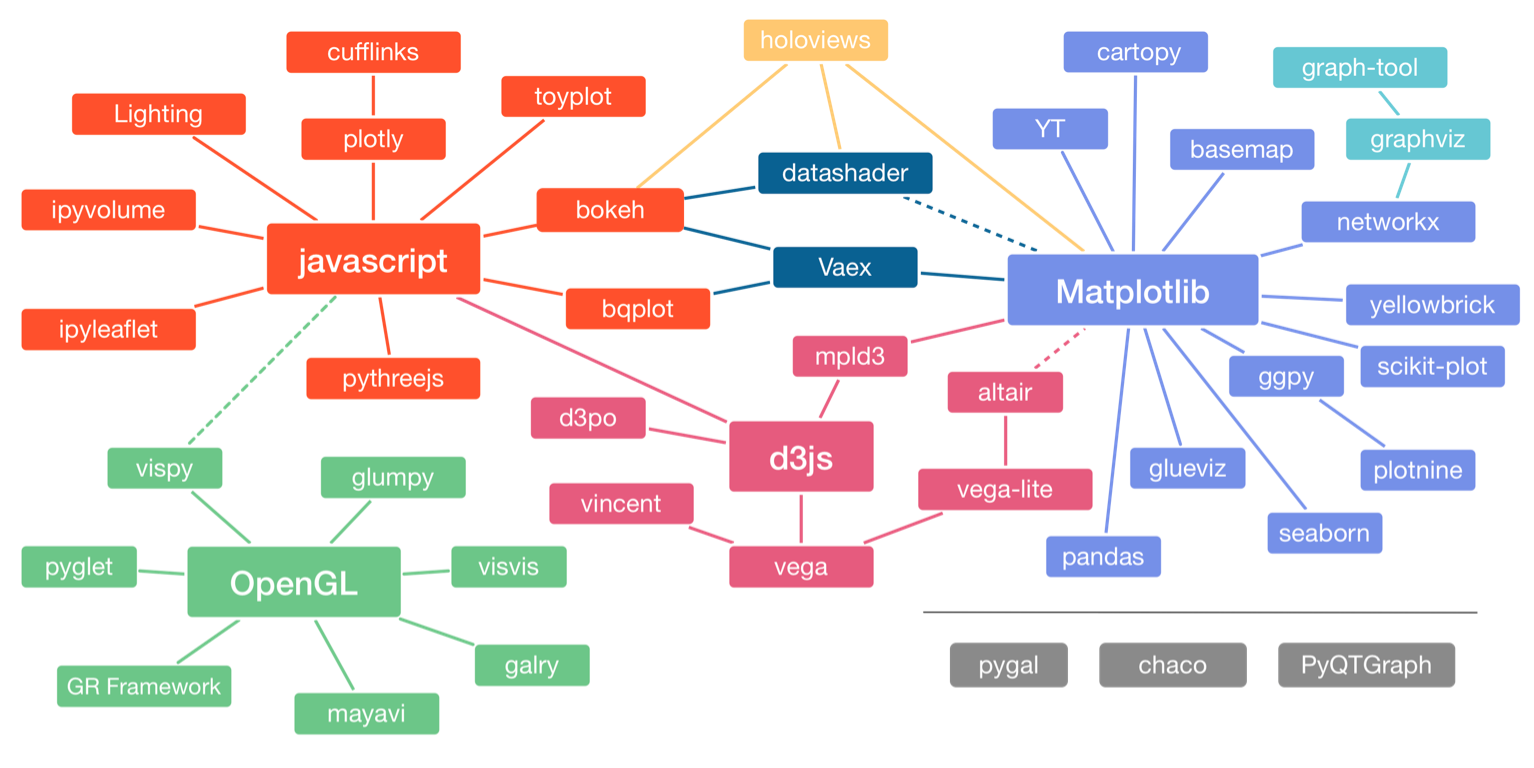
\includegraphics[height=0.8\textheight]{images/dviz_overview}
\end{frame}

% =========================== Bibliography =================================
\begin{frame}
	\frametitle{References}
	\printbibliography
 \end{frame} 

\end{document}